\documentclass[5p]{elsarticle}
\usepackage{lineno,hyperref}
\modulolinenumbers[5]
\journal{Journal of Network and Computer Applications}

\usepackage{amsmath,amssymb,amsfonts,chemarrow,balance,booktabs}
\usepackage{graphicx}
\usepackage{subfigure}
\usepackage{mathenv}
\usepackage{color}
\usepackage{multirow}
\usepackage{float}
\usepackage{threeparttable}
\usepackage[inline]{enumitem}
\usepackage{url}
\usepackage{hyperref}
\usepackage[linesnumbered,ruled,noend]{algorithm2e}
\usepackage{algpseudocode}
\usepackage{listings}
\usepackage{bytefield}
\usepackage[table]{xcolor}



\newcommand{\BfPara}[1]{{\noindent\bf#1.}\xspace}
\renewcommand{\baselinestretch}{0.96} 
\newcommand{\bc}{{Bitcoin}\xspace}
\newcommand{\rc}{{{\em RouteChain}}\xspace}
\newcommand{\bcc}{{Blockchain}\xspace}
\newcommand{\Bbc}{{Blockchain}\xspace}
\newcommand{\etc}{{etc.}\xspace}
\newcommand{\eg}{{\em e.g.}\xspace}
\newcommand{\ie}{{\em i.e.,}\xspace}
\newcommand{\cc}{{cryptocurrency}\xspace}
\newcommand{\Cc}{{Cryptocurrency}\xspace}
\newcommand{\cj}{{cryptojacking}\xspace}
\newcommand{\Cj}{{Cryptojacking}\xspace}
\newcommand{\bt}{{{\em BlockTrail}}\xspace}


\newcommand{\ddos}{{DDoS}\xspace}
\newcommand*{\defeq}{\stackrel{\text{{\color{brown}def}}}{=}}
\newcommand{\tsref}[1]{\textsection\ref{#1}\xspace}
\newcommand{\todo}[1]{{\color{red}{[TODO: #1]}}}
\newcommand{\etal}{{\em et al.}\xspace}
\newcommand{\parag}[1]{{\noindent\bf#1}}
\newtheorem{condition}{\textbf{Condition}}
\newtheorem{theorem}{\textbf{Theorem}}
\newtheorem{claim}[theorem]{Claim}
\newtheorem{proposition}[theorem]{Proposition}
\newtheorem{lemma}[theorem]{Lemma}


\definecolor{xgreen}{rgb}{0.2,0.6,0.0}
\definecolor{xred}{rgb}{0.7,0.1,0.0}
\def\equationautorefname~#1\null{(#1)\null}
\let\subsectionautorefname\sectionautorefname
\let\subsubsectionautorefname\sectionautorefname

\definecolor{light-gray}{gray}{0.95}
\definecolor{darkgray}{rgb}{0.4, 0.4, 0.4}
\definecolor{purple}{rgb}{0.65, 0.12, 0.82}
\definecolor{editorGray}{rgb}{0.95, 0.95, 0.95}
\definecolor{editorOcher}{rgb}{1, 0.5, 0} % #FF7F00 -> rgb(239, 169, 0)
\definecolor{editorGreen}{rgb}{0, 0.5, 0} % #007C00 -> rgb(0, 124, 0)
\definecolor{orange}{rgb}{1,0.45,0.13}      
\definecolor{olive}{rgb}{0.17,0.59,0.20}
\definecolor{brown}{rgb}{0.69,0.31,0.31}
\definecolor{purple}{rgb}{0.38,0.18,0.81}
\definecolor{lightblue}{rgb}{0.1,0.57,0.7}
\definecolor{lightred}{rgb}{1,0.4,0.5}

\usepackage{amsmath}

\newcommand\JSONnumbervaluestyle{\color{blue}}
\newcommand\JSONstringvaluestyle{\color{blue}}
\newif\ifcolonfoundonthisline
\makeatletter


\lstdefinestyle{json}
{ backgroundcolor=\color{light-gray},
    basicstyle=\footnotesize\ttfamily,
    showstringspaces=false,
    breaklines=true,
    frame=lines,
  showstringspaces    =false,
  keywords            = {false,true},
  commentstyle= \itshape\color{codegreen},
  alsoletter          =0123456789.,
  morestring          = [s]{"}{"},
  stringstyle         = \ifcolonfoundonthisline\JSONstringvaluestyle\fi,
  MoreSelectCharTable =%
    \lst@DefSaveDef{`:}\colon@json{\processColon@json},
 % basicstyle          = \ttfamily,
  keywordstyle        = \ttfamily\bfseries,
}


\newcommand\processColon@json{%
  \colon@json%
  \ifnum\lst@mode=\lst@Pmode%
    \global\colonfoundonthislinetrue%
  \fi
}


\hypersetup{
	plainpages=false,
	colorlinks,
	urlcolor=blue!50!black,
	linkcolor=red!50!black,
	citecolor=green!50!black,
	bookmarksnumbered
}


\bibliographystyle{elsarticle-num}

\begin{document}
\begin{frontmatter}
\title{RouteChain: Towards Blockchain-based \\Secure and Efficient BGP Routing}
\author[]{Muhammad Saad}
\ead{saad.ucf@knights.ucf.edu}
\author[]{Afsah Anwar}
\ead{afsahanwar@Knights.ucf.edu}
\author[]{Ashar Ahmad}
\ead{ashar@cs.ucf.edu}
\author[]{Hisham Alasmary}
\ead{hisham@Knights.ucf.edu}
\author[]{Murat Yuksel}
\ead{Murat.Yuksel@ucf.edu}
\author[]{Aziz Mohaisen\corref{mycorrespondingauthor}}
\cortext[mycorrespondingauthor]{Corresponding author}
\ead{mohaisen@cs.ucf.edu}
\fntext[myfootnote]{This paper is an extension of an earlier work that appeared in IEEE International Conference on Blockchain and Cryptocurrency (ICBC 2019)~\cite{saad2019routechain}}



\address{University of Central Florida}


\begin{abstract}
Routing on the Internet is defined among autonomous systems (ASes) based on a weak trust model where it is assumed that ASes are honest. While this trust model strengthens the connectivity among ASes, it also results in an attack surface that can be exploited to hijack the routing paths. One such attack is known as the BGP prefix hijacking, in which a malicious AS broadcasts IP prefixes that belong to a target AS, thereby hijacking its traffic. In this paper, we propose \rc: a blockchain-based secure BGP routing system that counters BGP hijacking and maintains a consistent view of the Internet routing paths. Towards that, we leverage provenance assurance and tamper-proof properties of blockchains to augment trust among ASes. We group ASes based on their geographical (network) proximity and construct a bi-hierarchical blockchain model that detects false prefixes prior to their spread over the Internet. We evaluate \rc using three different consensus protocols and show its effectiveness by drawing a case study with the Youtube hijacking of 2008. Our results show that \rc can efficiently detect false prefix announcements and prevent BGP attacks over the Internet.    
\end{abstract}

\begin{keyword} Blockchain; Autonomous Systems; BGP; Distributed Systems\end{keyword}
\end{frontmatter}

\section{Introduction}\label{sec:introduction}
Data flows on the Internet between autonomous systems (ASes), which are connected in a peer-to-peer (P2P) topology~\cite{SpotoGM14,KanzakiF13}. Typically, an AS represents a collection of Internet Protocol (IP) prefixes, and to which data is routed~\cite{PadmanabhanL2001}. Due to P2P architecture, ASes require an effective communication protocol to maintain updated routing paths and monitor network changes. The semantics of this communication among ASes are determined by a standardized routing protocol called the Border Gateway Protocol (BGP) \cite{SermpezisKDD18}. Although efficient in practice, BGP is broadly based on a weak trust model, whereby ASes assume that their neighboring ASes behave honestly and propagate correct routing information. However, sometimes interests of ASes (i.e., networking operators managing them) can be in conflict, and this weak notion of trust can be breached by malicious ASes. As a result, this opens the door for attacks whereby malicious ASes may attempt to hijack the traffic of a target AS. A well-known attack that captures this exploitation of trust is known as the ``BGP prefix hijacking'' or simply the BGP hijacking~\cite{MitsevaPE18,JonkerPDS18}. 

In BGP hijacking, a malicious AS announces fake (impersonated or unreachable) IP prefixes that belong to a target AS. Conforming to the expectations of honesty and trustworthiness, neighboring ASes accept those prefixes and modify their routing paths for reachability. They further propagate the prefixes to their neighboring ASes. As the BGP announcement traverses across ASes, they update their routing tables according to the values in the announcement. Eventually, as the routing converges, the traffic destined for the legitimate AS---an AS that owns the announced prefix---gets diverted to the malicious AS, thereby causing a traffic hijacking. The redirected traffic does not reach the correct destination, thereby causing revenue and reputation losses. 



Although various solutions have been proposed to preventing the BGP prefix hijacking attacks, including BGPSec and RPKI, those solutions have not been deployed widely in practice~\cite{QiuGRN07}, making these attacks possible for the Internet's critical functionality of routing. A key reason behind this is that these solutions take a clean-slate approach towards redesigning routing protocols and policies, by introducing additional infrastructure for their operation. However, due to the capital invested in the existing Internet infrastructure, ASes and ISPs are reluctant to migrate towards these solutions despite the known security threats and their clear benefits. 

% This is a major inhibition in migrating towards a new protocol scheme which would require a system-wide overhauling of current Internet architecture. Therefore, ISPs and ASes continue to function in the conventional ways despite security risks.  

Embracing the policy-based functional challenges as well as the security risks in routing, we propose a new scheme called \rc, which counters BGP hijacking by leveraging design constructs of blockchains. Blockchains have introduced secure and robust ways of augmenting trust in distributed systems. Through secure-by-design protocols, blockchains enable tamper-proof data management without the need of a trusted intermediary. ASes broadly reflect a distributed mesh of interconnected systems, that often lack consensus over correct protocol execution. It is therefore intuitive to bring blockchain to the design space of ASes management in order to upgrade their security while maintaining operational consistency. \rc explores the usefulness of blockchains for BGP. 

In \rc, we treat a BGP announcement as a transaction, and {\color{blue} record each announcement an immutable blockchain ledger shared among the peers (ASes). To maintain a consensus over the blockchain ledger, ASes execute a consensus protocol which specifies the {\em correct} blockchain state and prevents malicious announcements. Blockchain systems use various consensus protocols to maintain the blockchain consistency, including Proof-of-Work (PoW), Proof-of-Stake (PoS), Proof-of-Authority (PoA), and Proof-of-Elapsed Time (PoET) \etc. In \rc, we deploy PoA, PoS, and PoET and evaluate their performance in preventing the BGP hijacks~\cite{BanoSAAMMD17,Angelis18,SaadSNKSNM20}.    

The premise of our work relies upon a consensus agreement among ASes, prior to the launching of an attack. To that end, we contrast the timings of known BGP attack on Youtube, with the consensus time in \rc. Our results show that while all consensus protocols meet the baseline requirement of preventing the attack, in particular, Clique (a PoA-based protocol) achieves the lowest transaction confirmation time and the maximum transaction throughput.} \rc is incrementally deployable and backwards compatible with the current operations of ASes. ASes can use it in parallel with their current routing policies as an additional security feature. Therefore, \rc does not require ASes to switch from legacy systems to a new protocol paradigm. 


\BfPara{Contributions} We make the following contributions:
\begin{enumerate*}
    \item We introduce a blockchain-based system called \rc that prevents BGP hijacking.
    \item We set up a testbed in different ASes across the world and evaluate \rc's performance under three blockchain consensus protocol. 
    \item Our experiments show that \rc can neutralize a BGP hijack attempt in all three consensus protocols. Among them, we note that Clique achieves the best performance due to minimum transaction confirmation latency. 
    \item We further demonstrate the feasibility of \rc by drawing a case study from the well-known Youtube's BGP hijacking case, where \rc is shown to neutralize the attack.  
    \item Our proposed solution is shown to be incrementally deployable; easily implemented alongside existing protocols. 
\end{enumerate*}

\BfPara{Organization} The rest of the paper is organized as follow. In \textsection\ref{sec:bg}, we provide the background and preliminaries of our work. In \textsection\ref{sec:ps}, we introduce the problem statement, the threat model, the motivation, and the methodology. In \textsection\ref{sec:rc}, we present our proposed solution \rc, along with its design and analysis. In \textsection\ref{sec:simulation}, we present the simulations and results. In \textsection\ref{sec:discussion}, we discuss the advantages and limitations of our work. That is followed by related work and conclusion in \textsection\ref{sec:rw} and \textsection\ref{sec:conclusion}.  




\section{Background and Preliminaries}\label{sec:bg}
In this section, we briefly review the background of ASes, BGP, and blockchains, aligned with the scope of this work. 

\subsection{Autonomous Systems and BGP} \label{sec:AS}
\BfPara{ASes} The Internet is composed of interconnected entities that forward data from a source to a destination. These entities can range from small local area network (LAN) switches, ASes that connect geographically distributed communication devices and networks. 

An AS is a collection of connected routers whose IP prefixes are assigned to an Internet Service Provider (ISP). These routers adhere to the routing policy defined by the ISP. Every AS on the Internet is assigned a unique Autonomous System Number (ASN), which is used as an identifier in inter-AS, a.k.a. inter-domain, routing. An AS is responsible for routing the traffic among networks hosted by itself and other networks hosted by its neighboring ASes. For that, an AS uses the Interior Gateway Protocol (IGP) to enable communication among its internal routers attached to networks it is hosting, and the Exterior Gateway Protocol (EGP) to reach the routers in the neighboring ASes. Inter-AS relationships are established according to economic or business relationships among ISPs owning ASes. The relationship between two neighboring ASes can be peering or customer-provider engagement, and typically means that a level of trust exists between them.  
%(peers, customers, or providers). Each router maintains routing tables to identify and monitor routing paths. 


\BfPara{BGP}
The Border Gateway Protocol (BGP) is a standard protocol that is designed to connect edge routers between two neighboring ASes. BGP enables the propagation of reachability and routing information from one AS to another~\cite{rfc4271}. It is also used for routing information within the AS itself. BGP operates in two ways: It uses interior BGP (iBGP) for routing among the network peers within an AS, and the external BGP (eBGP) for routing to/from other ASes~\cite{rfc4271,SmithG96}. In this paper, we are concerned with eBGP that pivots communication among edge routers of neighboring ASes. \autoref{fig:ASes} shows the connection of routers within and outside the ASes. The bold circles represent the edge routers that are connected to either the internal or external routers through the BGP protocol. %%what's the difference between 

\BfPara{BGP Attacks}\label{bgp:attacks}
The exploitation of trust among neighboring ASes leads to BGP attacks. These attacks can be broadly classified into two types: partial attack and complete attack~\cite{BGPHijack}. The partial attack occurs when an adversarial AS announces an identical IP prefix as that of the victim AS. One such attack was launched on Youtube on February 24th, 2008, by an ISP that owned AS17577~\cite{BiersackJFFTTTV12,WongS11}. AS17577 started to announce the prefix 208.65.153.0/24---which actually belonged to the Youtube AS36561---to its upstream provider AS3491. AS3491 further propagated the prefix to its neighboring ASes, leading to the Youtube hijacking. In the partial hijacking, the adversary has no significant advantage over the victim. Since the two announcements are the same, therefore when any AS receives the announcement, it can either switch to it or continue with the old routing path. 

In complete attacks, the adversarial AS announces more specific prefixes than the target AS. Since the default forwarding scheme is based on longest prefix matching, ASes switch to more specific prefixes. Therefore, when an adversary announces more specific prefixes, any AS that receives the announcement inevitably switches to the new routing path. Therefore, in this attack, the adversary has a significant advantage over the victim~\cite{BGPHijack}.The upside in this attack is that the adversary can only hijack a portion of the traffic destined to an AS since it has to announce a longer prefix.

\begin{figure}[t]
\begin{center}
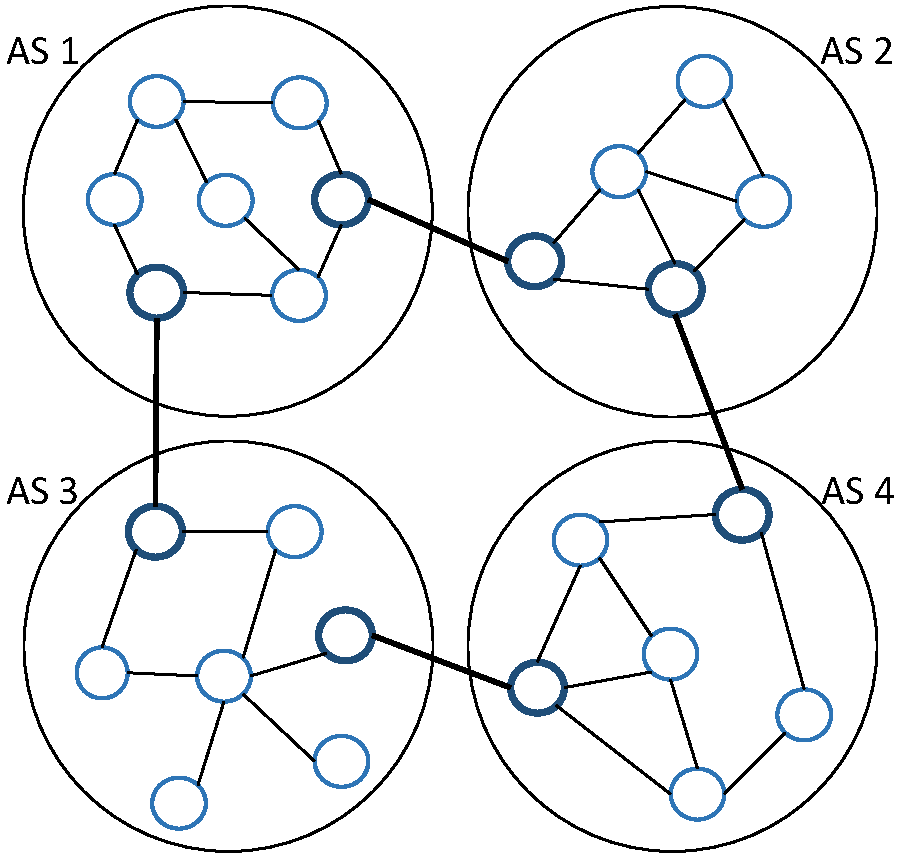
\includegraphics[width=0.30\textwidth]{fig/ASes.pdf}
%\vspace{-12mm}
\caption{An overview of ASes connected to one another. In AS 1--4, the circles inside represent routers that are responsible for intra-AS routing. Bold circles represent the border routers that are connected to other border routers through BGP protocol. To emphasize their connectivity, we color them in dark.  } 
\label{fig:ASes}
\end{center}

\end{figure}


\subsection{Blockchains} \label{sec:BC}
Blockchain technology has introduced a new paradigm in distributed systems with applications spanning cryptocurrencies, smart contracts, distributed provenance, and censorship resistance~\cite{NeisseSN17,Omohundro14,GovernatoriIMRS18,AhmadSBM18}. With promising guarantees including immutable and append-only data management in a decentralized system, blockchains are well suited to create provenance and prevent fraud in a trust-less environment. 

Blockchains use various consensus protocols to arbitrate trust among networks and entities. Some of the well-known consensus protocols include the proof-of-work (PoW), proof-of-stake (PoS), proof-of-elapsed time (PoET), proof-of-authority (PoA), and the practical Byzantine fault tolerance (PBFT) \cite{SaadM18,SaadNKM18}. Each scheme has its merits and caveats. However, best suited to the requirements of our design, we use a modified form of PoA, known as {\em Clique}. For more details on consensus schemes and their uses, we refer the reader to \cite{Bano:2017b}.

% While PoW is highly scalable, it is energy inefficient and suffers from low throughput. On the other hand, BFT achieves high throughput, but it has low scalability, and high message complexity. However, specific to the requirements of \rc, we envision that BFT can be effectively tailored to meet the design goals of our system. 



\begin{figure}[t]
\centering
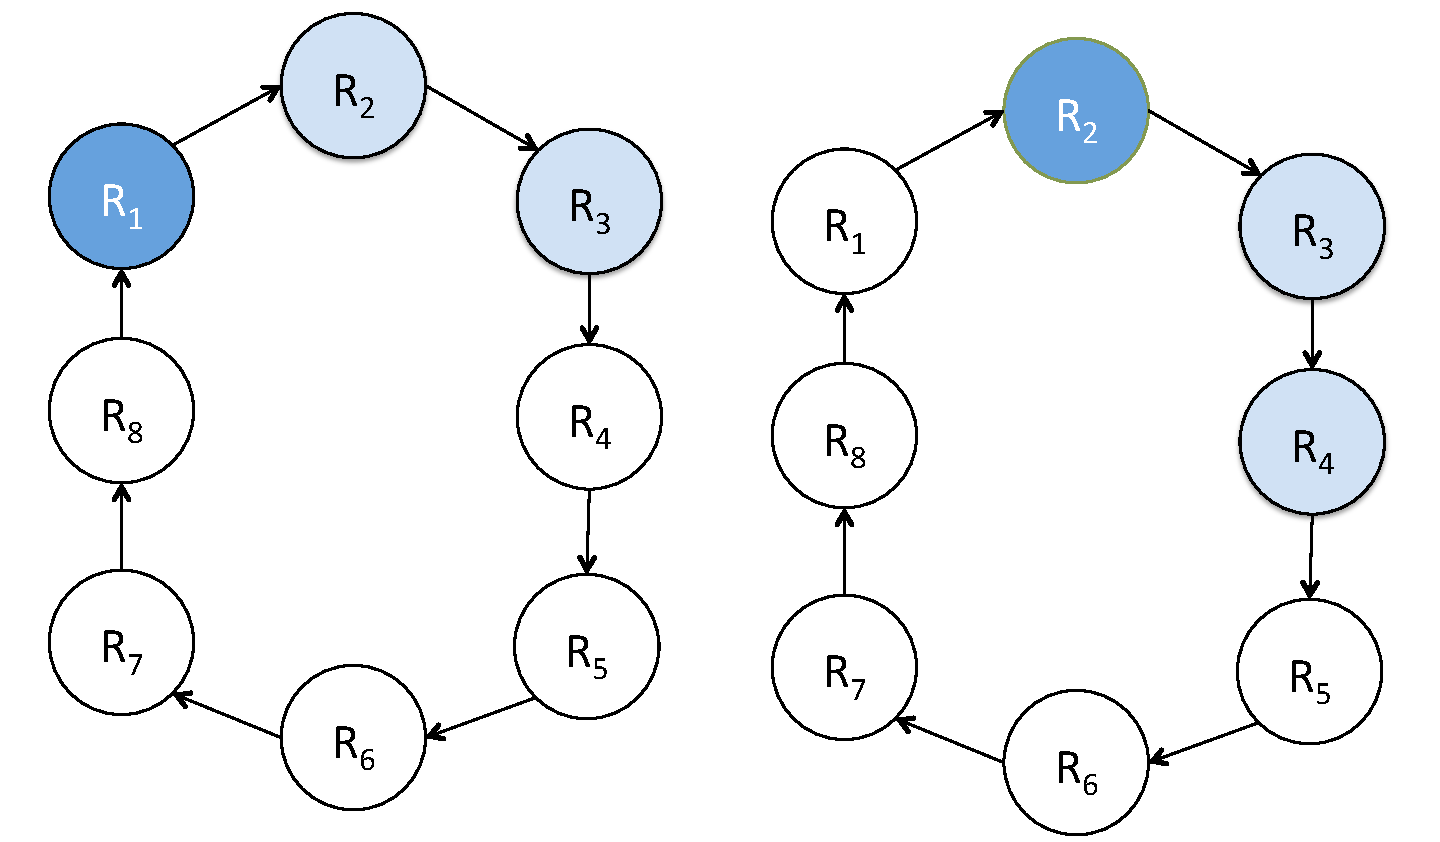
\includegraphics[width=0.45\textwidth]{fig/bgp_clique_roundrobin.pdf}
%\caption{  Selection of ASes responsible to propose blocks in Clique. The ASes are selected in a round-robin fashion with a primary and a set of secondary nodes such that each AS is only allowed to propose a block every $N/2 + 1$   } 
\caption{Clique uses a round-robin scheme to select primary node, and two secondary nodes, the primary is responsible for proposing a new block. In case of failure of a primary node the block is proposed by the secondary nodes. Note: R1 is the primary and R2 and R3 and secondary for the first epoch, for the second epoch R2 is the primary and R3 and R4 and the secondary. }
\label{fig:Clique}
\end{figure}


\BfPara{{\em Clique}} \label{sec:cq}
{\em Clique} is a PoA-based consensus scheme that is fast, scalable, and has high fault tolerance. In {\em Clique}, a primary is chosen to order transactions and broadcast to the nodes for each round of block execution. In contrast to PBFT, where block execution takes four phases with $O(n^2)$ message complexity, a block is executed in a single phase with $O(1)$ message complexity in {\em Clique}. For each epoch, a primary replica is selected in a round-robin, and the view of the primary is replicated on the mutually shared ledger. Moreover, {\em Clique} has a high fault tolerance and can endure up to $f/2$ faulty replicas. In \autoref{fig:Clique}, we show how a primary replica is selected in {\em Clique}, and later in \textsection\ref{sec:consen} we present the design implementation of {\em Clique} in our system. 

{\color{blue}{
\BfPara{{\em PoS}} \label{sec:pos}
PoS protocol addresses the energy inefficiency of PoW and replaces the computational requirements with the notion of stake in the system \cite{king2012ppcoin}. In PoS cryptocurrencies, the stake is the number of coins owned by a user, which are then used to make bids during a block auction process. The auction winner is allowed to propose a block. Due to the growing concerns about the energy consumption in PoW, cryptocurrencies including Ethereum are switching to PoS. Despite the obvious benefits, PoS has its limitations, including the problem of ``{\em the rich gets richer}'' \cite{BentovGM16}. The auction naturally favors rich miners who are rewarded with a transaction fee. As a result, their stake further increases which allows them to win the subsequent auctions as well. 

\BfPara{{\em PoET}} \label{sec:poet}
PoET protocol uses Intel Software Guard Extensions (SGX) to execute the ``leader election'' code in a secure enclave. Each blockchain node executes the code, generate a random wait time during which the node remains idle. Once the wait time expires, the node is allowed to propose a block~\cite{chen2017security}. PoET randomizes the leader election process to maintain decentralization. In contrast, PoW and PoS may become centralized if a node acquires an exceptionally high hash rate or has a high balance for auction. Currently, Hyperledger Sawtooth supports the PoET protocol \cite{Sawtooth}.
}}

\section{Problem Statement and Threat Model}\label{sec:ps}
In the following, we describe our problem statement along with the threat model. Using this model, we build the motivation and describe the methodology of our work.

\subsection{Problem Statement} \label{sec:psn}
Broadly speaking, the problem with routing attacks on ASes involves the exploitation of a weak trust model that parameterizes the communication among ASes. Each AS has its own routing table at the the gateway router, which only includes routing information of the ASes that are directly connected to it. Moreover, when a new  piece of routing information is presented to the AS---that is not in conflict with its own routing policies---it readily accepts them and sets its outbound traffic to the new path. Moreover, the router at the gateway is unaware of the routing paths maintained by neighboring ASes. Lacking a global knowledge obstructs the detection of a malicious routing path when propagated. Therefore, the lack of a synchronized global knowledge along with a weak trust model lead to the routing attacks. Although those attacks are infrequent, their impact could be catastrophic, making them important to address. 

Another challenge in preventing BGP hijacking is the cost associated with the existing countermeasures. For instance, one of the well-known countermeasures is the use of ``Resource Public Key Infrastructure'' (RPKI) \cite{rfc8481}, which enables network operators to cryptographically authorize ASes the to announce a specific prefix. To effectively use RPKI, ASes set up a route assigning authority called ``Routing Origin Authorization'' (ROA), that overlooks prefix authorization. While promising in theory, RPKI has some practical limitations. First, it requires all ASes to become part of a central authority and conform to its policies. In a decentralized network of over 80,000 ASes---each with a different functional policy---achieving this agreement can be challenging. Second, this clean-slate approach towards design and deployment of routing schemes may not be acceptable to network operators. 

\subsection{Threat Model} \label{sec:tm}
For BGP attacks, we assume the adversary to be a malicious AS or a group of ASes, aiming to hijack traffic of a target AS. The adversary can either launch a partial hijacking by announcing an identical prefix, or launch a complete hijacking by announcing more precise IP prefixes of the victim AS (\textsection\ref{bgp:attacks}). The adversary will exploit the weak trust model of its neighboring ASes, and expect them to change their routing paths accordingly. After announcement to the neighboring ASes, the adversary will hope its prefixes propagate swiftly through other ASes to maximize the attack severity. 

Assuming a victim is a valuable AS (i.e., an AS of interest to the adversary), hosting nodes that contain sensitive or valuable information, such as Bitcoin mining pools, then a large-scale attack can be launched to eclipse the target AS. In this attack, multiple ASes can simultaneously launch a complete or partial BGP attack, thereby hindering the recovery process of the victim. In such a situation, the attack may persist for a long time, causing excessive revenue and reputation loss~\cite{BangeraG11}.



\subsection{Motivation}\label{sec:motivation}
The motivation of this work is to introduce a blockchain-based routing scheme to prevent BGP attacks. We intend to use the tamper-proof guarantees of blockchains to equip routing tables with an immutable ledger that tracks routing paths. Therefore, when a malicious AS announces false prefixes, the rest of the network is able to detect and discard them. Moreover, keeping in view the need of a swift consensus, we aim to design \rc in a hierarchical way to improve performance and reduce latency. At the time of writing this work, there are 88,721 ASes on the Internet~\cite{RIR-18}, and using {\em Clique} to achieve consensus among them over a single routing path will lead to significant delays and unnecessary processing overhead. To avoid that, we intend to explore new design parameters that can be tailored to the efficiency requirements of the system.  Finally, a major effort in this work has been dedicated towards the incremental deployment of \rc: our objective is to achieve a standalone system that can be integrated with the current {\em Modus Operandi} of ASes and does not require them to modify their policies. 


\subsection{Methodology}\label{sec:method}
First we explore possible ways in which \rc can be structured to meet the requirements of {\em Clique}. We design our system in such a way that the consensus time among ASes is less than the time of hijacking. To that end, we set Youtube hijacking of 2008~\cite{GoldbergS14} as our baseline attack model to derive the hijacking time. Next, we compare the consensus time in \rc with the hijacking time obtained from the baseline attack model to analyze the strength of our design in adversarial settings. We do that by carrying event driven simulations that mimic the real-world conditions of the Internet. Since \rc is a modular structure, we tailor its design to achieve consensus over routes in minimum time. 




\section{\rc}\label{sec:rc}
In this section, we present the design and analysis of \rc. In \autoref{tab:one}, we provide the notations that will be used throughout the rest of the paper.  


{\def\arraystretch{1}
\begin{table}\caption{Symbols and Definition}
\centering
\scalebox{0.95}{
\begin{tabular}{l|l} 
\hline 
\textbf{Symbols} & \textbf{Definition} \\
\hline
$A$  & ASes in world $A = { a_{1},a_{2},...a_{n}}$\\
$K$  & ASes subgroups $K ={k_{1},k_{2},...,k_{p}}$, where $p\leq n$ \\ 
$\mathcal{A}$  &  A group of one or more adversarial ASes\\
$\mathcal{V}$  &  Victim AS to be hijacked by $\mathcal{A}$ \\
$\mathcal{B}_{A}$  &  Global blockchain for $A$\\ 
$\mathcal{T}_{A}$  &  Global blockchain consensus time for $\mathcal{B}_{A}$ \\
$\mathcal{B}_{K}$  & Subgroup blockchains, $\mathcal{B}_{K} {\mathcal{B}_{k_{1}},\mathcal{B}_{k_{2}},...\mathcal{B}_{k_{p}}}$  \\
$\mathcal{P}_{A}$ & Global primary replica for $\mathcal{B}_{A}$\\
$\mathcal{P}_{k_{i}}$ & Subgroup primary replica for $k_{i}$, where $1\leq i\leq p$\\
$\mathcal{T}_{K}$  & ASes consensus time in a subgroup \\
$\mathcal{T}_{A}$  & Consensus time in global blockchain \\
$\mathcal{T}_{E}$  &  End-to-end transaction delay \\
$\mathcal{T}_{h}$  &  Time to hijack target AS \\
$\mathcal{T}_{p}$  &  communication time between two ASes. \\
$\mathcal{T}_{v}$  &  Blockchain verification time \\
\hline
\end{tabular}}
\label{tab:one}
\end{table} } 

\subsection{System Architecture}\label{sec:do}
The overall design of \rc involves all ASes $A$ sharded into $K$ subgroups, with each subgroup sharing a single ledger. Subgroups are constructed based on their geographical proximity in order to reduce propagation delays and achieve faster consensus. Within a subgroup, each AS will maintain a subgroup ledger to keep track of routing paths that belong to all ASes within the subgroup. Having such a transparent and consistent view ensures that if any AS is targeted within the subgroup, all other ASes will be able to detect that, and take preventive measures. 

Our choice of sharding ASes into groups has multiple benefits. First, maintaining a single ledger for all ASes on the Internet can have a significant storage overhead, since each AS will be forced to maintain and update the routing information of all other ASes.  % Since routing paths are updated frequently, therefore, in an append-only model of blockchains, this would require a frequent update of ledger at each AS. % Furthermore, as the blockchain size will grow, the time to verify a new transaction will also increase. For a system of over 80,000 peers, having a single ledger would be computationally expensive along with an increasing storage overhead. 
Second, as the blockchain size grows, the time required to validate the correctness of a new transaction increases. For each new transaction, an AS would need to check the entire blockchain to view the prior history of a path defined in the new transaction. This verification time is critical, since it contributes to the overall consensus time. Having a long single ledger would increase the verification time for each incoming transaction. 

Finally, the key challenge in \rc is to obtain consensus of peers over a new route before the convergence of the legacy system. As mentioned in \textsection\ref{sec:motivation}, \rc will be deployed in parallel to the legacy system, therefore our objective is to flag a bogus route before it propagates through the legacy system and leads to a hijack. In \rc, subgroups will enable a parallel processing over a new transaction. Since ASes in subgroups are associated based on their geographical (network) proximity, they can achieve faster consensus due to low propagation delays for any given transaction. As such, parallel processing within subgroups will reduce the overall consensus time, as opposed to a flat blockchain system composed of all ASes. As such, sharding ASes in subgroups is a useful for fast consensus over BGP routes. 

For provenance assurance and a globally consistent view, \rc also maintains a global blockchain shared among subgroups. The global chain one maintains decisions on a given transaction, and does not contain detailed information of routing paths. For instance, when an AS announces his prefixes in a transaction, once the transaction gets approved by subgroups, the concerned subgroup updates its routing table while the global chain locks the transaction approval. The global chain will have all the announcements that are made by ASes in the form of a transaction. Therefore, when a new transaction is issued by an adversarial AS, the global blockchain can be consulted to track the true owner of those prefixes. The global chain however, does not include the routing paths that are maintained at the routers of an AS. 

In summary, \rc is a bi-hierarchical blockchain system, consisting of a global chain shared among subgroups, and subgroup chains shared among ASes. Once a transaction is generated, it is forwarded to subgroups, and upon receiving approvals, its status is updated in the ledgers (\textsection\ref{sec:SA}).   


\subsection{Subgroup Structure}\label{sec:sg}
% The subgroups are actuated based on their geographical locality. For instance, if we have to form two groups of ASes in \autoref{fig:ASes}, then ISP A, B, and C can form one group due to their spatial closeness, while ISPs E, F, and D, can form another group. These groups will have to blockchains to manage their routing paths. One blockchain will be local to the group of ASes, while the other blockchain will be global chain that will record the routes shared among all the groups of ASes. The subgroup size is adjustable to meet the timing constraint of consensus. 

A subgroup will consist of multiple ASes with a shared ledger of routing paths. The selection of ASes for a subgroup can be achieved through various design choices. For instance, grouping ASes based on their geographical proximity can reduce propagation delays. On the other hand, grouping them based on their transit relationships can have less policy conflicts. \rc is agnostic towards the policy of forming subgroups as long as each subgroup shares a single ledger. In this paper, we assume the peer relationship to be driven by the incentive of geographical proximity and low delays~\cite{rfc1930}. However, as part of our future work, we will explore other mechanisms to that be adopted for better results. In \autoref{fig:ASes_SG}, we illustrate how four ASes from \autoref{fig:ASes} can be arranged into two subgroups. 

In \textsection\ref{sec:mind}, we derive optimal value of the number of subgroups $K$, that results in minimum delays for consensus. Since the Internet architecture is continuously evolving and the network typologies change with time, therefore we accommodate this changing modularity in \rc by keeping the subgroup size and number of subgroups flexible. For instance, let $|k_{max}|$ be the upper size limit of a subgroup. If a group of new ASes falls into the same geographical proximity, and its addition would breach the size limit, then two subgroups can be extracted from the same subgroup.  




\begin{figure}[t]
\begin{center}
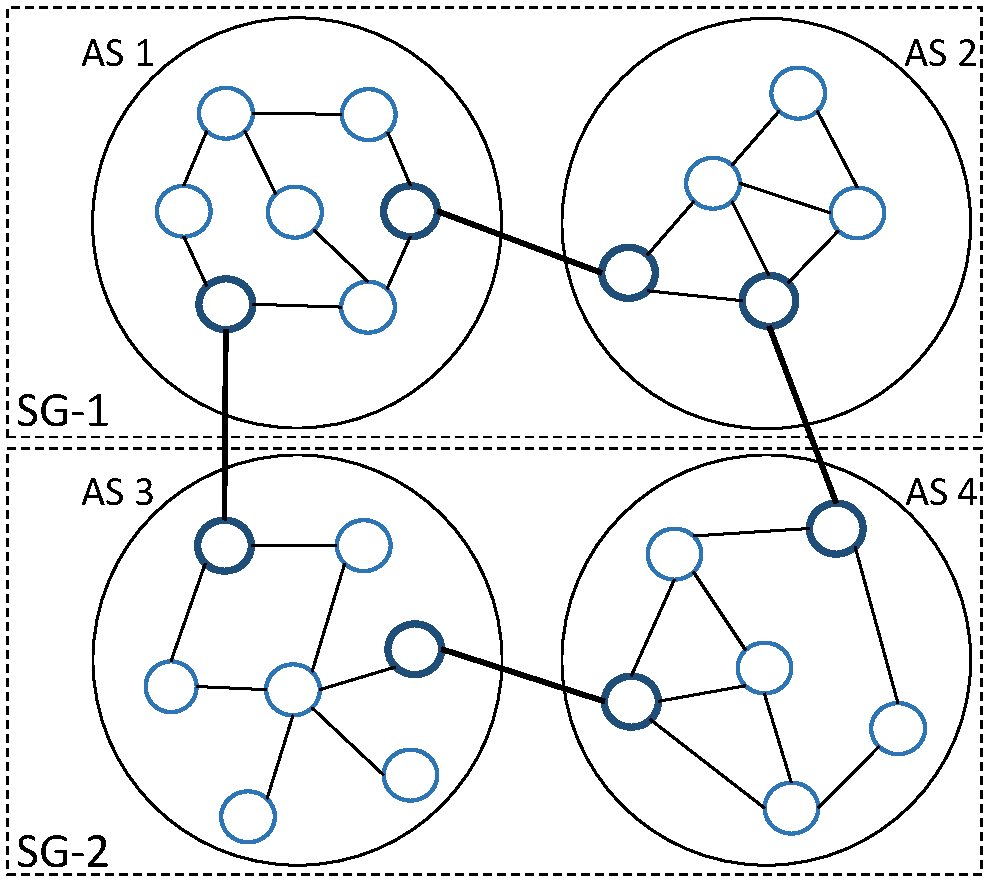
\includegraphics[width=0.30\textwidth]{fig/ASes_SG.pdf}
\caption{An overview of subgroup ASes. SG-1 is a subgroup with two ASes, AS 1 and AS 2 in close proximity. SG-2 is another subgroup of two ASes, AS 3 and AS 4 in close proximity. Selection of subgroups can be made on any other scheme such as transit route policy.} 
\label{fig:ASes_SG}
\end{center}
\end{figure}

\begin{figure}[t]
\begin{center}
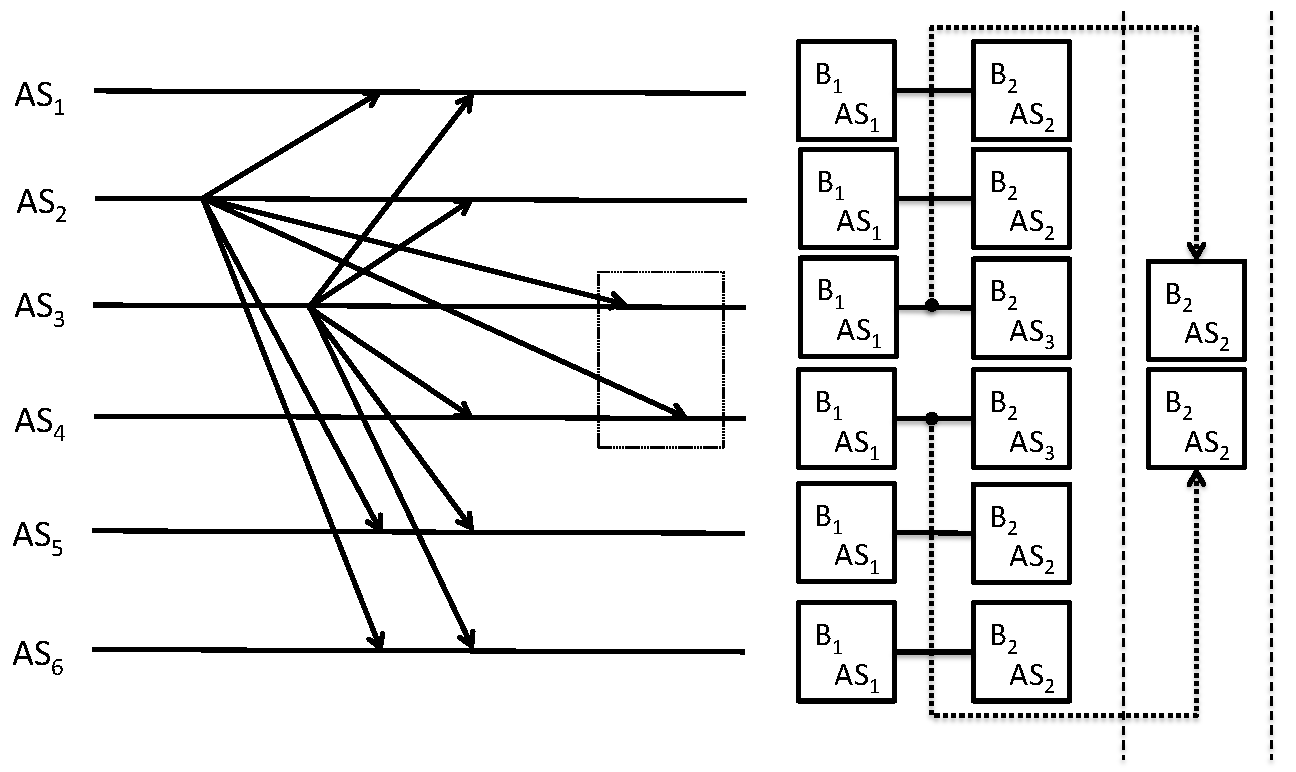
\includegraphics[width=0.45\textwidth]{fig/bgp_clique.pdf}
\caption{Fork in clique consensus protocol, $AS_2$ is the primary replica who broadcasts a block. Due to delays and latency  $AS_4$ does not get the block on time. Instead it receives the block published by the next primary $AS_3$. This leads to a fork. The fork can be resolved easily by mapping the prior known identity of the primary with the expected block. } 
\label{fig:Clique_fork}
\end{center}
\end{figure}

% ASes could be partitioned using a number of criteria, however to reduce the round-trip delay and contain a BGP attack in a geographical location, we propose we propose grouping ASes in geographical location in a group. So ASes in Central Florida would be in one group, and the ASes in North Florida will be in another group, and so on. We will be grouping optimal number of Ases in each group such that the number of ASes in group will be between $a_{max}$ and $a_{min}$, later on in the result section we will look into an optimal values of these parameters. 

% The internet is continuously evolving and the network structures changes, and more ASes or added or removed in a geographical region. To support these changes to network topology, out design automatically evolves and Ases are added or removed from the groups, and the groups can be merged and split to ensure a timely consensus among the blockchain peers. When the number of ASes in a group reach $a_{max}$ value the group is split into two groups, \eg if the ASes in Central Florida reach  $a_{max}$ value the group is split in two groups. On the other hand if the number of ASes go below the $a_{min}$ value, this group will be merged with a group geographically closest to this group. 

\subsection{Consensus Mechanism}\label{sec:consen}
As mentioned in \textsection\ref{sec:cq}, in \rc, we use {\em Clique} as the consensus protocol. For each subgroup in $K$, a primary replica $\mathcal{P}_{K}$ is selected to send transactions to other replicas (ASes) as shown in \autoref{fig:Clique_fork}. $\mathcal{P}_{K}$ is responsible for receiving transactions, ordering transactions, computing a block, and broadcasting it to the other replicas. This process is carried out in one epoch, and at each epoch, a new primary is selected to continue the procedure. The selection of a primary follows a round-robin scheme. Therefore, in a subgroup size of $|k_{i}|$, if an AS becomes the primary, it has to wait for $|k_{i}|-1$ epochs to become the primary again.  

% adding a new block to blockchain, once the block produced by primary replica is committed and the next AS take the responsibility to add the next block and this process continues in round robin manner and the, and the same primary replica is give this responsibility after $n-1$ blocks are added to the system, when n is the number of nodes in a subgroup.
%In \rc, for each subgroup in $K$, a primary replica $\mathcal{P}_{K}$ is selected to send transactions to other replicas (ASes). 

In {\em Clique}, it is possible that a block broadcasted by a primary gets does not reach all replicas in time. This can happen due to network delays or protocol malfunction. Moreover, it is also possible that in such non-deterministic network behavior, the block of the next primary arrives at a replica before the block of the current primary. This may lead to a disordered sequence of blocks or a fork, as shown in \autoref{fig:Clique_fork}. 

Resolving a fork in {\em Clique} is straightforward. Since the identity of the primary replica is known, therefore for each epoch, all ASes expect the new block with the identity of the primary replica, as shown in \autoref{fig:packet_bc}. Therefore, when blocks are received out of the order, replicas can resolve the forks and align their view of the blockchain. We illustrate this aspect of fork formation and resolution in \autoref{fig:Clique_fork}. 

% In \autoref{fig:Clique_fork}, a fork is taking place in clique, Primary authority $AS_2$ proposes a new block, and another non primary authority $AS_3$ also proposes a block new block, which results in a fork at $AS_3$ and $AS_4$. $AS_3$ and $AS_4$ detects the fork the subsequent block is received and the effected (ASes) would correct the fork by taking the correct block.

% Figure 3: A fork occurring in Clique. Authority a4 has the block proposed by a3 as second
% block, while a5 has the block proposed by a2. Eventually, a4 replaces the block proposed by a3
% with that proposed by a2 because the latter has a higher score.

% These transactions are BGP prefixes announced by an AS. Once the announcement is made, the primary replica receives it and sends it to all the replicas (ASes) within the group. These replicas consult their blockchain to see any routing conflicts. Assuming there are $f$ malicious replicas, in a subgroup, if the primary replica receives approval from $3f+1$ replicas, then it approves the transaction and appends it to the blockchain. 

% In the global blockchain, once the primary replica obtains approval from within the subgroup, it sends the group approval to the global primary replica. Assuming that there are $g$ faulty groups of ASes, if the global primary replica receives approval from $3g+1$ groups, it executes the transaction and appends to the global blockchain. 


\BfPara{Transaction Data Structure}\label{secc:tds}
In \autoref{fig:packet}, we show the data structure of transaction generated by an AS. The transaction consists of a transaction ID field, an autonomous system number (ASN) field, and the BGP packet. For details on the structure of BGP packet, we refer the reader to~\cite{rfc4271} Once this transaction gets approved, it is updated in the global blockchain ledger. 

% transaction packet, which consists of Id, which is a unique value, and we are using a GUID for it, Autonomous System Number(ASN) is a special number assigned by IANA that uniquely identifies an autonomous system, and BGP Packet, that is the complete BGP packet that was sent for this transaction, to look at the details of the packet we refer the reader to .

\begin{figure}[t]
\begin{center}
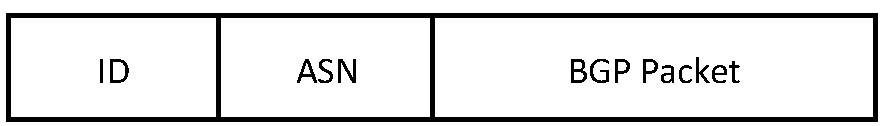
\includegraphics[width=0.40\textwidth]{fig/packet.pdf}
\caption{Transaction data structure in \rc. The unique identifier is used to for each transaction. Autonomous system number (ASN) field identifies the advertising AS, and BGP packet holds the metadata of routing information. } 
\label{fig:packet}
\end{center}
\end{figure}

\begin{figure}[t]
\begin{center}
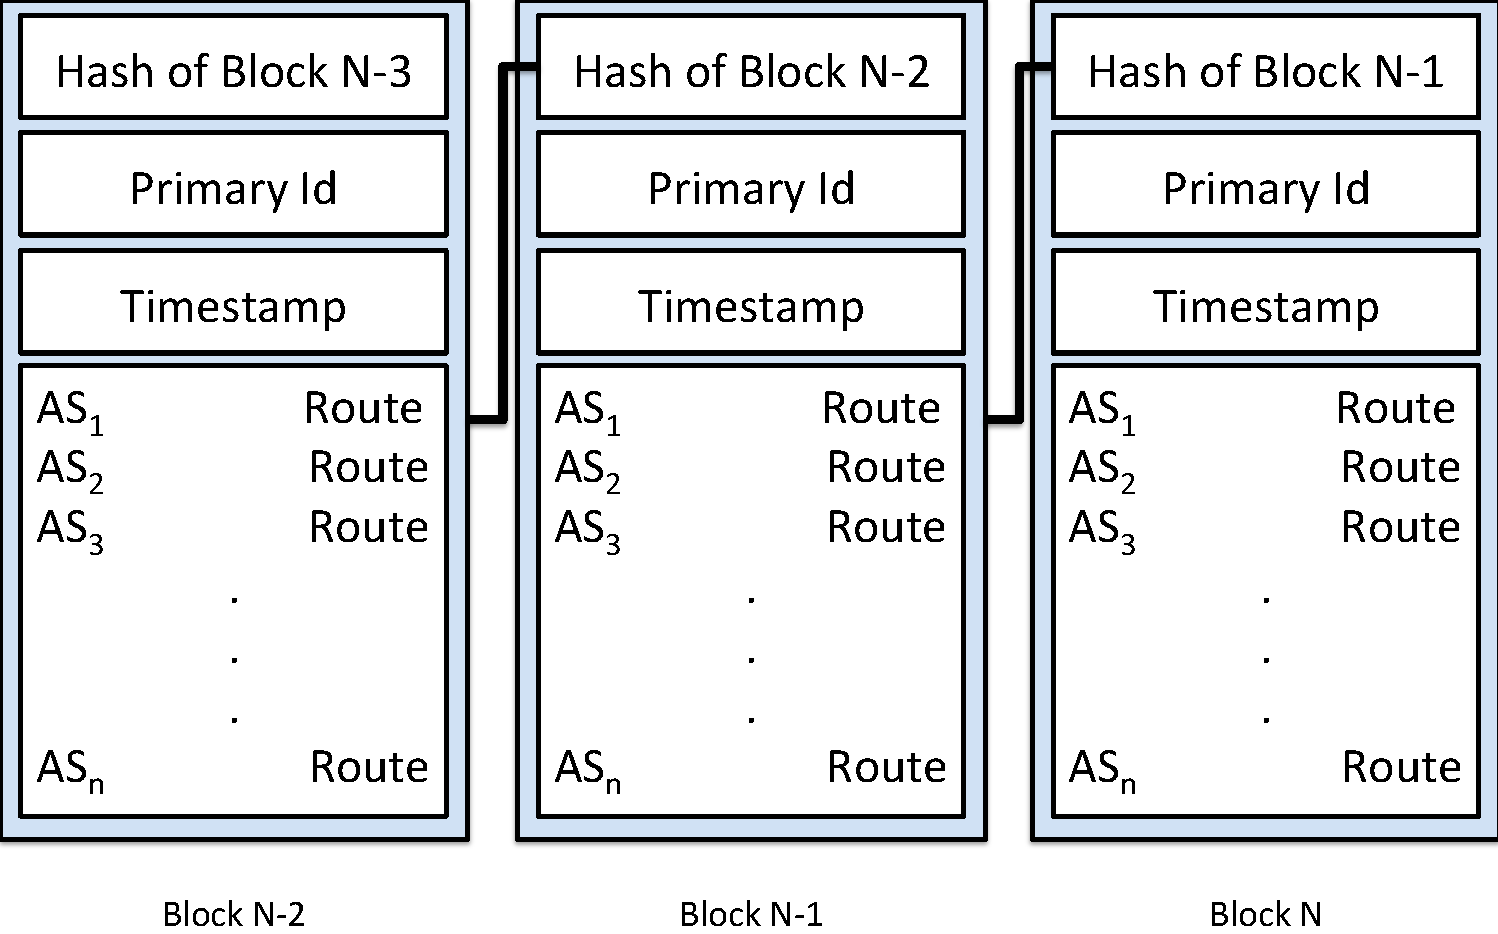
\includegraphics[width=0.40\textwidth]{fig/blockchain.pdf}
\caption{Blockchain data structure for a subgroup in \rc. The block contains a timestamp, hash of the previous block, and block payload. Block payload includes autonomous systems and their routes. All ASes within a subgroup have a transparent view of routes that belong to each AS. } 
\label{fig:packet_bc}
\end{center}
\end{figure}




\BfPara{Blockchain Data Structure}
In \autoref{fig:packet_bc}, we provide the structure of the blockchain for each subgroup. The blockchain consists of a timestamp that shows the time of block publication. The block also has a unique primary Id, and the hash of a previous block. In the block payload, we have all the ASes along with their complete routing paths. When a new block is computed, the routing paths are updated based on the newly approved transaction.

This blockchain data structure makes all ASes within a subgroup see all the BGP announcements. Based on import and export policies, the ASes may not want to re-advertise a path announcement. Also, an AS may do AS-PATH padding to increase the hop length of a path because it desires this path not to be used. But, our blockchain-based approach will effectively force all ASes in a subgroup to (i) re-advertise all the path announcements they received and (ii) use shortest possible paths. Although this may limit the flexibility in the import and export policies of individual ASes, it is an acceptable approach as the ASes in the same subgroup will likely trust each other and will not have an issue with sharing their prefix announcements. It is an open problem to design the blockchain data structure in a way that an AS advertising a path may choose to keep its announcement (or certain parts of it) encrypted while still adding it to blockchain for origin authorization purposes.






\subsection{Analysis of {\em RouteChain}} \label{sec:ana}
In this section, we perform analysis of \rc in terms of our design requirements and performance objectives. 
\subsubsection{Design Analysis}\label{sec:da}
In a {\em Clique} blockchain consisting of $N$ replicas, a transaction requires approval from $N/2$ replicas. In \rc, we make a minor adjustments to {\em Clique} such that the primary replica not only sends transactions to other replicas but also awaits an approval response. In the conventional design of {\em Clique}, the primary only broadcasts a transaction or a block and all other replicas accept the payload. However, suitable to our design, we expect other replicas to send back their approval for the transaction.

Additionally, the blockchain of a subgroup gets updated only if the approved transaction concerns the routing paths of ASes within the subgroup. Otherwise, only the subgroup decision is sent back to the global primary. We take this approach for two reasons. Firstly, a subgroup must only update its blockchain if a transaction directly concerns its routing path. Otherwise,  maintaining routing paths of other subgroups is an unnecessary overhead. Secondly, this also reduces the size of the blockchain, making transaction verification faster. 

The process of obtaining transaction approval involves:
\begin{enumerate*}
    \item An AS broadcasting transaction to its subgroup primary $\mathcal{P}_{K_{i}}$,
    \item $\mathcal{P}_{K_{i}}$ forwarding transaction to the global primary $\mathcal{P}_{A}$,
    \item $\mathcal{P}_{A}$ broadcasting transaction to all subgroups $K$, 
    \item $\mathcal{P}_{K_{i}}$ obtaining at least $|k_{i}|/2$ responses from subgroup replicas,
    \item and $\mathcal{P}_{A}$ obtaining responses from $|K|/2$ subgroups
\end{enumerate*}

For consensus within a subgroup, the primary will take one propagation delay $\mathcal{T}_{p}$ to broadcast the transaction to all replica ASes. Each AS will take the verification time $\mathcal{T}_{v}$ to verify transaction from the blockchain, and $\mathcal{T}_{p}$ to send back the response to the primary. However, due to varying link conditions and verification capacities, the overall time of receiving $|k_{i}|/2$ responses might incur non-uniform delays. We characterize such delays with parameter  $\epsilon_{1}$. Therefore, for a given transaction, the consensus time $\mathcal{T}_{K}$ of a subgroup can be calculated as follows: 
\begin{align} \label{eq:1}
    \mathcal{T}_{K} = \mathcal{T}_{p} +  \mathcal{T}_{v} + \mathcal{T}_{p} + \epsilon_{1} = \mathcal{T}_{v} + 2\mathcal{T}_{p} + \epsilon_{1}
\end{align}


In the second phase of transaction confirmation, the global primary $\mathcal{P}_{A}$ needs to obtain $|K|/2$ responses from subgroup primaries. Similar to \autoref{eq:1}, the time to achieve this consensus would be the verification time, the propagation time, and the second overhead $\epsilon_{2}$, capturing random delays for information propagation between subgroups and the global primary. Therefore, the transaction confirmation time $\mathcal{T}_{A}$, for the global blockchain $\mathcal{B}_{A}$ can be calculated as follows:
\begin{align}\label{eq:2}
    \mathcal{T}_{A} = \mathcal{T}_{K}+ \mathcal{T}_{p}+\epsilon_{2} = \mathcal{T}_{v} + 3\mathcal{T}_{p} + (\epsilon_{1}+\epsilon_{2})
\end{align}



In a complete transaction life cycle, the transaction will start from an AS within a subgroup and through will reach the global primary through the subgroup primary. Once received, the the global primary will initiate the verification process by broadcasting transactions to all subgroups. Taking into account propagation delays at each step, the end-to-end duration of a transaction $\mathcal{T}_{E}$ can be calculated as follows: 

\begin{align}\label{eq:3}
    \mathcal{T}_{E} = 3\mathcal{T}_{p} +\mathcal{T}_{K}+ \mathcal{T}_{A} = \mathcal{T}_{v} + 6\mathcal{T}_{p} + (\epsilon_{1}+\epsilon_{2})
\end{align}

 


\BfPara{Minimizing Delay}\label{sec:mind}
To defend against BGP attacks, we want the value of $ \mathcal{T}_{E}$ to be small. From \autoref{eq:3}, it can be observed that propagation delays  $\mathcal{T}_{p}$ linearly contribute the most towards the end-to-end duration of transaction confirmation $\mathcal{T}_{E}$. Therefore, in order to reduce the number of propagation delays, we need to reduce the number of messages required to process a transaction. This depends upon the number of ASes in a subgroup, and the total number of subgroups respectively. We know that in {\em Clique}, $N/2$ messages are required by the primary to commit a transaction (\textsection\ref{sec:consen}). This means that $\mathcal{P}_{A}$ requires approval from 50\% replicas in both hierarchies. If we fix, $K$ subgroups for \rc, the size of each subgroup will be $A/K$, and the number of approvals required will be $A/2K$, since approvals among the subgroups will happen in parallel. Next, $\mathcal{P}_{A}$ also require approvals from $K/2$ subgroups for the global blockchain. Therefore, for a transaction confirmation, in total, $\mathcal{P}_{A}$ requires $A/2K + K/2$ approvals. For simplicity, we assume that each subgroup is uniform in size such that $|k_{1}|=|k_{2}|=|k_{p}|$. Using that and after simplification, we obtain the following equation that shows the total number of approvals required for the transaction commitment $\mathcal{C}$. 
\begin{align}\label{eq:4}
\mathcal{C} = \frac{A }{2K} + \frac{K}{2}= \frac{A + K^{2}}{2K}
\end{align}

From \autoref{eq:4}, our objective is to find the suitable value of $K$ that yields minimum value of $\mathcal{C}$. Therefore, by differentiating \autoref{eq:4} with respect to $K$, and setting it to $0$, we obtain the optimum value of $K$ as:  $K^* = \sqrt{A}$.  Note that $K^*$ is independent of the fact that Clique requires half of the ASes to respond. This simplifies the design and $K^* = \sqrt{A}$ becomes an optimum target as the AS count $A$ changes. After plugging $A$ = 88,721, the total number of ASes in the world, we get $K^* \approx$ 298. This means that with number of subgroups fixed at 298, we will need minimum number of approvals for a transaction commitment. Minimum approvals will naturally have minimum propagation delays, which serves our main goal in \rc. 

\subsection{Security Analysis}\label{sec:SA}
In this section, we will analyze security properties of \rc in the light of the threat model. An adversary controlling one or more ASes will try to launch a partial or complete BGP attack on a target AS. In the following, we show how \rc defends against these attacks. 

\BfPara{Partial Attack} In a partial hijacking attack, the adversarial AS $\mathcal{A}$ announces identical BGP prefix that belongs to the victim AS $\mathcal{V}$. In the taxonomy of blockchains, this attack can be considered as double-spending, since $\mathcal{A}$ is trying to utilize a resource that is already being consumed by $\mathcal{V}$. As shown in \autoref{fig:packet}, the transaction will have the same BGP packet as payload but a conflicting value in ASN field. Since the global blockchain $\mathcal{B}_{A}$ will have a prior transaction of same prefixes linked to the identity of $\mathcal{V}$, such an anomaly can be easily detected in \rc. 

If $\mathcal{V}$ and $\mathcal{A}$ belong to the same subgroup, the hijacking attempt will be neutralized immediately by the subgroup primary $\mathcal{P}_{K_{i}}$, unless $\mathcal{A}$ is itself the primary. In such a case, the transaction will be sent to the the global primary $\mathcal{P}_{A}$. Also if $\mathcal{A}$ and $\mathcal{V}$ belong to different subgroups, the transaction will be forwarded to the $\mathcal{P}_{A}$ by $\mathcal{P}_{K_{i}}$. In both cases, the subgroup primaries will consult the global blockchain $\mathcal{B}_{A}$, and be able to spot the double-spent transaction. To defend against partial attacks, the response from subgroup primaries would be sufficient to obtain consensus over the transaction. As long as 50\% of the subgroup primaries behave honestly, a partial hijacking can be detected and countered immediately.  

\BfPara{Complete Attack} In a complete attack, $\mathcal{A}$ announces more specific prefixes than the ones owned by $\mathcal{V}$. As such, this behavior cannot be immediately detected as a double-spent transaction since $\mathcal{B}_{A}$ will not have a prior transaction linked to $\mathcal{V}$ that contains prefixes announced by $\mathcal{A}$. To detect that, \rc would require a conflict resolution from all ASes in subgroups. Each AS will consult their subgroup blockchain to see if the newly advertised routes in the transaction alters their routing paths. If true, they will observe the original path and its corresponding prefix. Next, they will locate the true owner of the prefix through the global blockchain $\mathcal{B}_{A}$. Accordingly, they will be able to detect that the newly announced prefix does not belong to the true owner, therefore, it is malicious. As long as 50\% ASes in a subgroup and 50\% of total subgroups behave honestly, the hijacking attempt can be detected and prevented in time. 

\begin{figure}[t]
\begin{center}
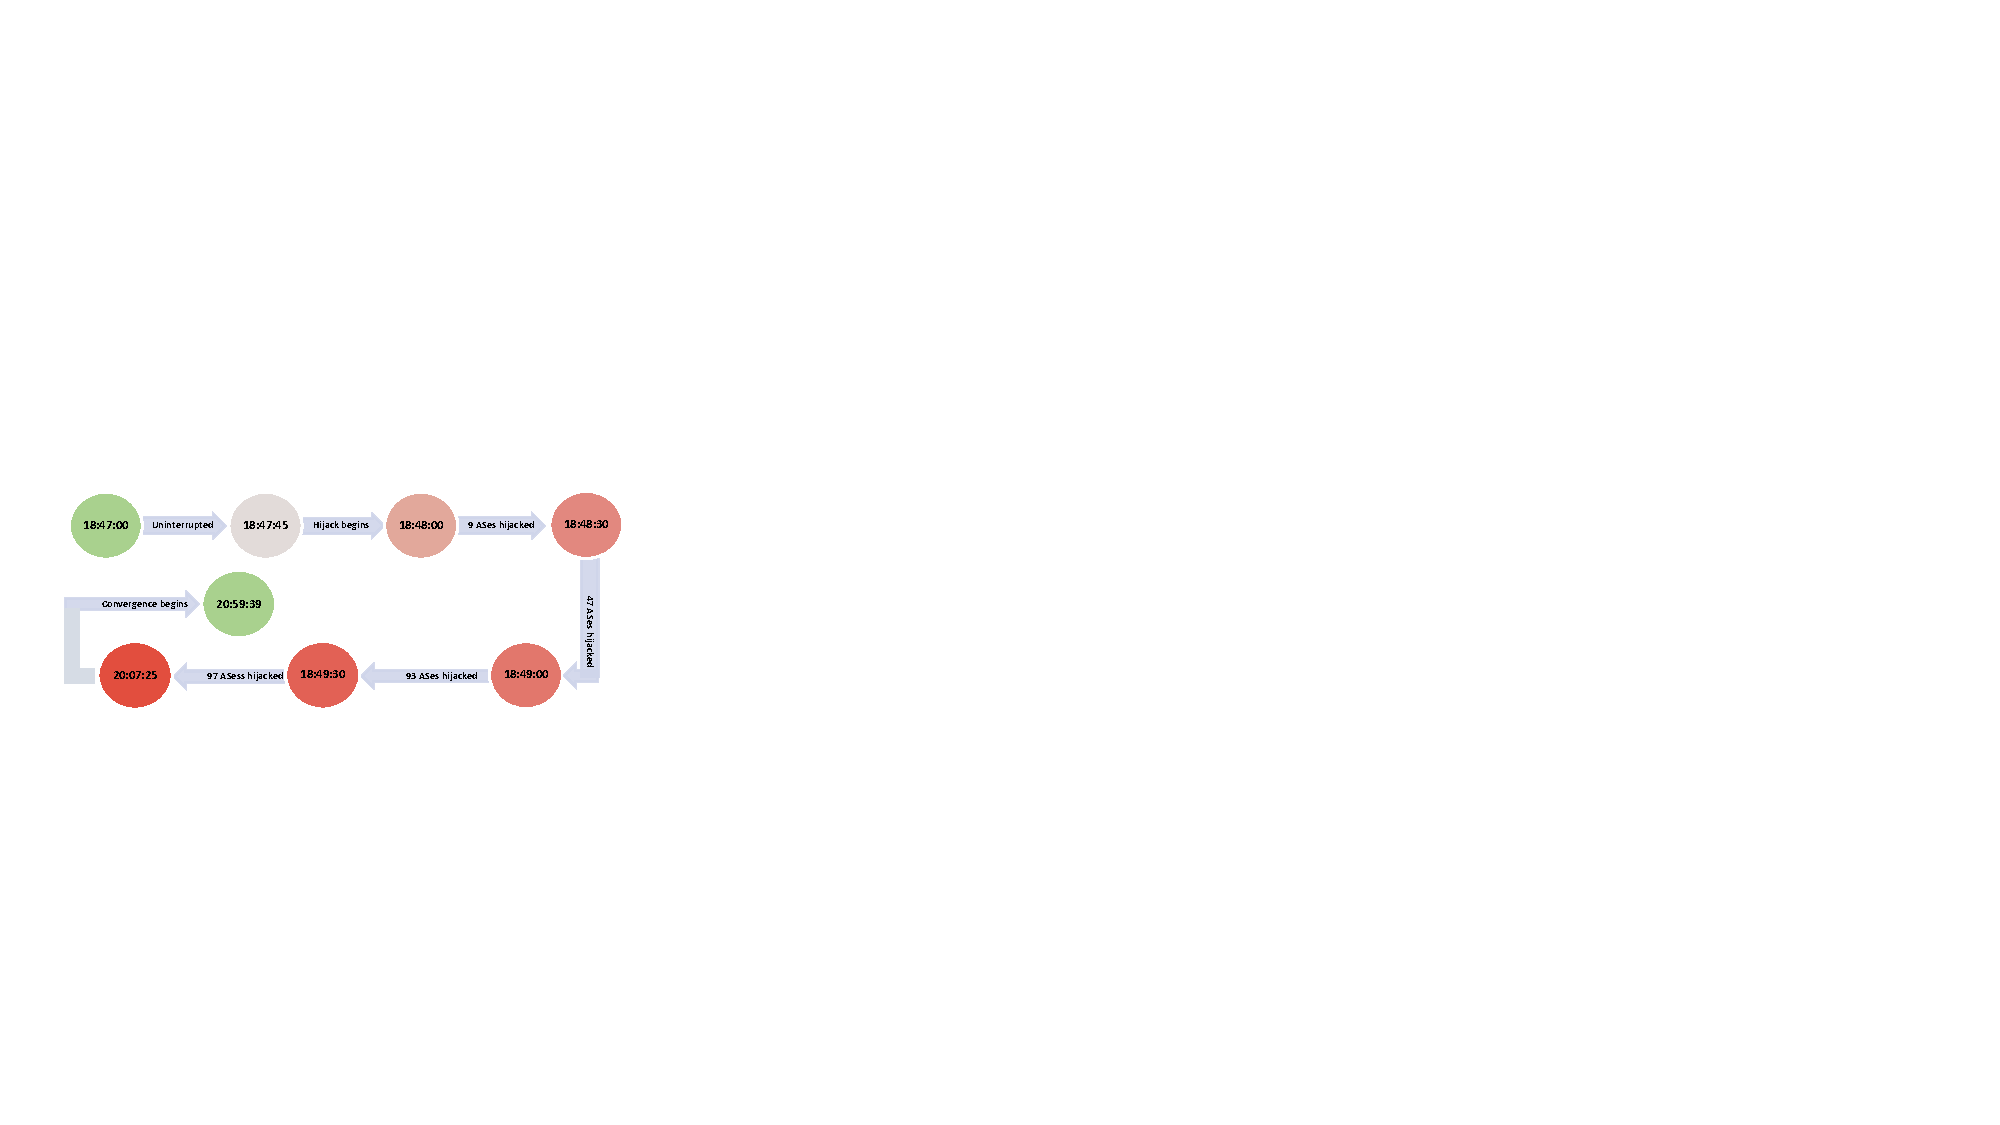
\includegraphics[width=0.45\textwidth]{fig/123.pdf}
%\vspace{-12mm}
\caption{Timeline of Youtube Hijacking. Notice that within one minute of the announcement, 9 ASes had changed their routes, and within 20 minutes 97 ASes were redirecting their traffic to AS17577.} 
\label{fig:YThijack}
\end{center}
\end{figure}

Compromising 50\% of ASes within a subgroup can be costly in practice. In all the well-known attacks that have been launched against ASes, only one AS or ISP has been found to be the miscreant. Therefore, in practical settings, even if the subgroup size is small, a collusion of 50\% ASes is highly improbable. Furthermore, the adversary will also need support from 50\% of the total number of subgroups. Therefore, for a successful attack, the adversary would require half of the total ASes in the world to be on its side. Considering the associated cost, we conclude that \rc provides high security guarantees in adversarial settings.  


% As shown in \textsection\ref{secc:tds}, we model the BGP packet as an ``Unspent Transaction Output'' (UTXO) transaction. Each prefix is locked with its corresponding AS, and if due to a change in the policy, the owner AS wants to assign its prefix to another AS, it will have to generate a new transaction that validates its ownership and shift ownership to the recipient AS. UTXO transaction ensures that a transaction input is fully consumed, meaning that a new prefix assignment invalidates the previous assignment. Additionally, in UTXO model, two transactions consuming same input are considered double-spent transactions. Therefore, in a partial hijacking, if an adversary generates a transaction that contains exact BGP prefix belonging to another AS, it can be treated a double-spent transaction. 

% Consider a situation in which an adversarial AS $\mathpzc{a}_{x}$ attempts to hijack another AS $a_{x}$, where both ASes belong to the same subgroup ($\mathpzc{a}_{x}, a_{x} \in k_{x}$). $\mathpzc{a}_{x}$ will generate a transaction from consuming the UTXO of the owner $a_{x}.$ His transaction will be immediately rejected by the rest of the peers in the subgroup $k_{x}$. The only way the attacker might succeed is if he controls more than half of the ASes in the subgroup ($|k_{x}|/2 \in \mathcal{A}$). 

% Now consider a situation in which an adversarial AS $\mathpzc{a}_{x}$ in subgroup $k_{x}$, tries to hijack an AS $a_{y}$ in subgroup $k_{y}$. Firstly, this would require $\mathpzc{a}_{x}$, to be the primary replica in $k_{x}$, in order to convey transaction to the global primary replica. The adversary will not broadcast transaction within its own subgroup ${k}_{x}$, since all peers will easily detect that $\mathpzc{a}_{x}$ is not the true owner of the prefixes announced in the transaction. Once the global primary $\mathcal{P}_{A}$ will forward transactions to other subgroups. Each subgroup will consult the global blockchain to see check if there is a previous owner of prefixes announced in the transaction. If 50\% subgroups behave honestly, the transaction will be rejected. 

% In the interest of time, a policy of {\em subgroup agreement before global agreement}, can be enforced to raise the attack cost. For a new transaction, the subgroup primary would be required to first obtain the consensus within the subgroup before forwarding it to the global primary. In which case, partial hijacking can be detected locally. 





% Let $A$ be the set of all autonomous systems over the Internet, where $A = {a_{1},a_{2},...,a_{n}}$. Let $B$ be the set of subgroups composed out of $A$, such that $B={b_{1},b_{2},...,b_{k}}$, where $B\in A$, and $k<n$.  For the common case, we assume the size of each subgroup in $B$ is equal, meaning that $|b_{1}| = |b_{2} = |b_{k}|.$  Let $\mathcal{L}_{bi}$ be the blockchain of an individual subgroup, and let $\mathcal{L}_{g}$ be the global blockchain. Let $t_{i}$ be the consensus time for a specific subgroup, and $t_{g}$, be the consensus time over the global blockchain. 

% From \autoref{fig:PBFT}, we can observe that within a subgroup, the transaction starts from the primary replica, passes through four stages, and finally goes to the client. In each stage, each replica performs verification of the transaction and sends a response back. If we assume $f(x)$ to be a function that computes end-to-end delay in transaction verification and for a single replica $x$ within a subgroup $y$, then the aggregate time for $3f+1$ replicas $T_{l}$ can be computed as $T_{l} = \min\limits_{x \in y} f(x)$. This means that $T_{l}$ is the time taken by the $3f+1$'st replica, which is the minimum end-to-end transaction verification time. 

% Now assume $T_{g}$ to be the time taken by the global primary replica to obtain response from $3f+1$ subgroups. As such, $T_{g}$ can be computed as $T_{g} =  \min (T_{l_{1}}, T_{l_{2}}, ..., T_{l_{3f+1}})$. This means that global confirmation time is the minimum time in which the global primary replica receives a response from $3f+1$ subgroups. 

% Once a BGP route is announced by an AS, its subgroup primary replica sends it to the global primary replica, as well as other ASes within the subgroup. The global primary replica sends the BGP route to all other subgroups, and obtains their consent. Once the global primary replica has sufficient confirmations, the route is processed and updated in the global blockchain. Additionally, each subgroup updates its local blockchain accordingly. Now, in attack conditions, if the consensus over a false prefix is achieved prior to the route acceptance in conventional scheme, then the attack can be prevented.
\section{Simulation and Results}\label{sec:simulation}
In this section, we present simulations and experiments performed to validate our theoretical analysis. In particular, we focus on achieving quick consensus over a malicious route announcement. Since \rc will be deployed in parallel with the existing infrastructure, it will not mitigate the attack completely. Instead, within few seconds, we expect \rc to notify all ASes about the validity of the announced prefix. Once notified, ASes can discard the announcement to prevent further propagation, and curtail damages. Towards that, we draw parallels with the {\em YouTube} Hijacking of 2008, and show how \rc is able to provide effective countermeasures.  

\begin{figure}[t]
\begin{center}
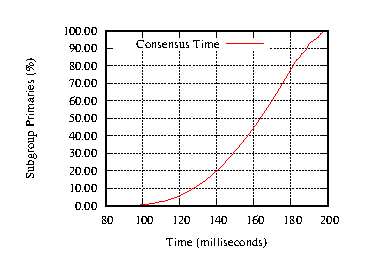
\includegraphics[width=0.45\textwidth]{fig/partialHijackR2.eps}
\caption{Consensus time of subgroups during a partial hijacking. Notice that the network is able to detect the malicious broadcast within 200 milliseconds. } 
\label{fig:simPartial}
\end{center}
\end{figure}

\begin{figure}[t]
\begin{center}
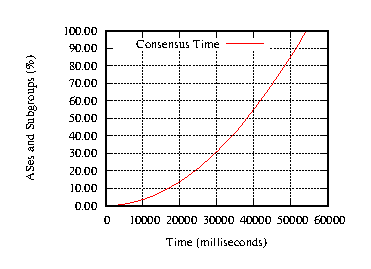
\includegraphics[width=0.45\textwidth]{fig/completeHijackR2.eps}
\caption{Consensus time of subgroups during a complete hijacking. Subgroups and their ASes are able to detect the attack within 54.23 seconds.} 
\label{fig:simComplete}
\end{center}
\end{figure}



Based on the design principle to reduce the time and message complexity, we consider the following parameters in our design: (1) the subgroup size $A/K$, (2) the number of subgroups forming the global blockchain $K$, (3) the subgroup consensus time $\mathcal{T}_{K}$, (4) the global blockchain consensus time $\mathcal{T}_{E}$, and (5) propagation and verification delays. 




We formulate simulations based on \autoref{eq:1}--\autoref{eq:3}, and we take practical values of AS propagation delays and blockchain verification time from the prior work~\cite{LabovitzABJ01,TakahashiEII15,pazmino2015}. Using these values, we set parameters in our simulator and model subgroup consensus and global consensus. Consensus time in a subgroup is the round-trip time from the transaction broadcast till the approval of $|k_{i}|/2$ replicas. For simulations, we record the time taken to receive a confirmation from each AS. Therefore, the consensus time becomes the difference between the start time of transaction broadcast and the time taken to receive acknowledgement from the last expected AS. Similarly global consensus time is the time taken to receive the acknowledgment from the slowest subgroup. 
%Similarly, for the time for global consensus is the round-trip time for to receive acknowledgement from the last subgroup. 

% global-chain round-trip time is the time taken to form a consensus of a subgroup of ASes with the global chain, which is dependent on the last subgroup to receive an acknowledgement from.

Next, we analyze the effectiveness of \rc, in the light of our threat model \textsection\ref{sec:tm}. In a  partial hijack, only the consensus from the subgroup primaries is sufficient to detect the hijacking attack and neutralize it. Since the partial hijacking attack reflects a double-spending attack in the global blockchain, subgroup primaries can effectively query the blockchain and notify the global primary. To that end, we simulate this scenario and show the consensus among subgroups over a malicious route in \autoref{fig:simPartial}. It can be observed that for a partial hijacking attack, the consensus is achieved within 200 milliseconds. 

To prevent a complete hijacking attack, \rc acquires consensus of subgroups and ASes within a subgroup. We simulate that by recording the round-trip time between subgroup primaries and their ASes, and the round-trip time between the global primary and subgroup primaries. We plot our simulation results in \autoref{fig:simPartial}. It can be noticed that a complete hijacking attack can be detected within 54.24 seconds. Although, the consensus time over the complete hijacking attack is higher than the partial hijacking attack, considering the timings of real world attacks, this is tolerable. 

To further evaluate the effectiveness of \rc, we contrast the consensus time with the timings of Youtube's attack. In \autoref{fig:YThijack}, we provide the timeline of the attack. It can be observed that during the attack duration, within 1 minute, 9 ASes were hijacked and within 20 minutes, 97 ASes were hijacked. Therefore, considering the short consensus time of \rc, we can assert with confidence that our system will notify the ASes about the attack while it is in its initial stages. Network operators can configure their rotuers to switch back to old routes once an attack is detected. 

% To observe the real time application and usability of \rc, we compare the convergence of \rc with the hijacking propagation in case of {\em YouTube}{'s} BGP hijacking by {\em Pakistan Telecom} in 2008. It can be seen that by the time the protocol leads to hijacking of almost 2 ASes, \rc creates a consensus among all the ASes.
\section{Discussion}\label{sec:discussion}
As shown by simulation, \rc is able to expose the BGP announcements to all ASes in 54.24 seconds. More specifically, for a partial hijacking, as outlined in \autoref{fig:YThijack}, \rc is able to obtain consensus from all ASes within 200 milliseconds. If \rc was deployed by ASes during the Youtube hijacking, it would have been able to prevent the hijacking when only 4 ASes were compromised. This could have saved traffic and revenue loss for Youtube AS. 

Since \rc is a standalone service that runs in parallel with the operations of an AS, it cannot completely prevent all ASes from attack. Consensus among ASes is a function of time (\autoref{eq:1}--\autoref{eq:3}), and as such, transaction propagation and verification among all ASes may take some time. As a result, the threat of a hijacking cannot be completely eliminated even with \rc, however, as shown by simulations, the damage prevention is significant.

One limitation of our work is the assignment of ASes within subgroups. To achieve ideal results, we show how subgroups can be structured to obtain consensus in minimum time (\autoref{eq:4}), however, in practice this may not be as close to the ideal situation. We group ASes based on geographical proximity. However, in the real world~\cite{LiangBXH11}, ASes may have conflicting interests or policies that may prevent them from being part of the same subgroup that also contains their competing ASes. However, as we mentioned earlier, geographical proximity is one policy, among others, that be used to construct \rc. As such, subgroup structure is agnostic of the underlying policy as long as it shares a single ledger. Furthermore, a subgroup size can vary depending upon its construction policy. While obtaining consensus from 50\% ASes is pertinent to the transaction verification, however, reducing their number will reduce the latency. A transaction can be processed with agreement of fewer replicas, provided that the system has a strong trust model. We view this as an avenue for future research where the performance of \rc can be evaluated based upon varying subgroup size, structure, and policy. Finally, \rc can be incrementally deployed from a small group of ASes to all ASes over the Internet. In this paper, we provide a roadmap towards secure routing through immutable route management. This can be bootstrapped at a small scale and later adapted by entities which find it useful. 


\section{Related Work}\label{sec:rw}
In this section, we review notable efforts done to secure Internet routing protocols against well known attacks. Towards blockchain-based secure BGP routing Xing~\etal\cite{XingWW18} proposed  {\em BGPcoin}; a smart contract driven BGP framework that is implemented over Ethereum network. {\em BGPcoin} reduces the possibility of BGP prefix hijacking by providing secure BGP advertisements through smart contract enabled authentication. Hari \etal~\cite{HariL16} also proposed a blockchain-based secure BGP routing. They also identified caveats in using RPKI in the decentralized architecture of ASes. However, their proposal did not include a design blueprint that can be effectively used among ASes. Chang~\etal\cite{ChangVWKLSL11} proposed a behavioral assumption scheme, called {\em AS-TRUST} to design ASes reputation. {\em AS-TRUST} provides probabilistic trust for the ASes by evaluating their prior broadcasts and classify the outcomes based on a reputation function. Towards blockchain-based secure Domain Name Systems (DNS), Liu~\etal\cite{LiuLCHXW18} proposed a data storage method, called DecDNS that creates multiple DNS nodes in parallel to address single point-of-failure in DNS resolution. 

There has been extensive research carried out to secure BGP without the use of blockchains. Hu~\etal\cite{HuWL15} proposed Cooperative Information Sharing Model (CoISM) to improve shortcomings of information sharing through BGP monitoring. CoISM does not modify the current processing of BGP and can be implemented to validate real BGP routes and detect fake BGP routes. Moreover, it can be deployed in various inter-domain management applications, such as intrusion detection and failure analysis of routing. Camacho~\etal\cite{CamachoGBV13} proposed BGP eXtended Multipath (BGP-XM) for transit Autonomous Systems. BGP-XM uses algorithms including K-Best Route Optimizer  to strengthen BGP multi-path routing. BGP-XM does not violate BGP functionalities when selecting routes among different ASes paths. Schlamp~\etal\cite{SchlampHJCB16} proposed a ``Hijacking Event Analysis Program'' {\em HEAP}; to filter data sources and rate validity of BGP sub-prefixes in order to defend against hijacking. 

% To justify our choice of using the consensus scheme for blockchain application, we consulted work done by Bano~\etal\cite{BanoSAAMMD17}, that explores all popular consensus schemes including proof-of-work, proof-of-stake, and Byzantine fault tolerance. They evaluated the performance of each scheme using various parameters such as scalability, throughput, and security. From that, we derived our motivation to use BFT for our work. 

% Ahmad~\etal\cite{AhmadSBM18} proposed a blockchain-based solution to secure audit logs against the physical access attack and the remote vulnerability attack. To that end, they used BFT protocol to augment consensus among the untrusted parties that are associated with audit log applications. They used a property appraisal application provided by Clear Village Inc. to model their design and experimented with varying payload size.




\section{Conclusion}\label{sec:conclusion}
In this paper we present a blockchain-based secure BGP routing system called \rc. \rc uses a bi-hierarchical blockchain structure and {\em Clique} consensus protocol to facilitate fast and tamper-proof route management. While the blockchain ledger provides a validation source for all prefixes, {\em Clique} enables swift consensus among ASes over the nature prefix broadcast. Combined, these two properties enable \rc to act as standalone security service that can be incrementally deployed in parallel with current operations of ASes. We validate achievable objectives of \rc through discreet-event simulations, and our results show that \rc can effectively curtail a BGP attack while it is in its initial stage.  


\BfPara{Acknowledgement:}This work is supported by Air Force Material Command award FA8750-16-0301 and Global Research Lab program of the National Research Foundation NRF-2016K1A1A2912757.




\bibliography{references.bib,conf.bib}




\end{document}

